\documentclass[a4paper,11pt]{article}
\usepackage{amsmath, amssymb, graphicx, siunitx, subcaption, float, booktabs}
\usepackage[margin=1in]{geometry}
\usepackage{titlesec}
\usepackage{physics}
\usepackage{xcolor}
\usepackage{caption}

\title{\textbf{Rectangular Waveguide Design}}
\author{Amirkahshayar Maghsoud }
\date{}

\begin{document}

\maketitle

\section{Introduction}
This report presents the analysis using the data mentioned below for the rectangular waveguide:
\[
a = 0.1080~\text{m}, \quad b = 0.0831~\text{m},\quad L = 0.05~\text{m} \quad a > b, \quad  \varepsilon_r=3, \quad \text{Mode} = \text{TE}_{2,4}
\]
the length of the waveguide, $L$, has been assumed to be $50~\text{mm}$ in order to minimize the margin of error between the CST and MATLAB simulations. Additionally, the thickness of the PEC wall, denoted as $h$, has been set to $0.001~\text{m}$ in the CST simulation to accurately represent the waveguide boundaries.

\section{ Cutoff Frequencies of Propagating Modes}
Starting from the longitudinal field equation for TE/TM modes:
\[
\nabla_t^2 H_z + k_c^2 H_z = 0
\]
where \( k_c^2 = \left( \frac{m\pi}{a} \right)^2 + \left( \frac{n\pi}{b} \right)^2 \),
the cutoff frequency is:
\[
f_{c_{mn}} = \frac{c}{2\pi \sqrt{\varepsilon_r}} k_c = 
\frac{c}{2\sqrt{\varepsilon_r}} 
\sqrt{\left( \frac{m}{a} \right)^2 + \left( \frac{n}{b} \right)^2}
\]
\noindent\textbf{Note:} For compactness, only TE modes are listed in the table. 
However, whenever both mode indices $m$ and $n$ are nonzero ($m,n \ge 1$), 
a corresponding TM$_{m,n}$ mode also exists with the \emph{same cutoff frequency}. 



\begin{table}[H]
\centering
\caption{Cutoff frequencies of propagating TE modes up to and including TE$_{2,4}$}
\small
\begin{minipage}[t]{0.49\textwidth}
\centering
\begin{tabular}{cccc}
\toprule
Mode & $m$ & $n$ & $f_c$ [GHz] \\
\midrule
TE$_{1,0}$ & 1 & 0 & 0.8013 \\
TE$_{0,1}$ & 0 & 1 & 1.0414 \\
TE$_{1,1}$ & 1 & 1 & 1.3140 \\
TE$_{2,0}$ & 2 & 0 & 1.6026 \\
TE$_{2,1}$ & 2 & 1 & 1.9113 \\
TE$_{0,2}$ & 0 & 2 & 2.0829 \\
TE$_{1,2}$ & 1 & 2 & 2.2317 \\
TE$_{3,0}$ & 3 & 0 & 2.4040 \\
TE$_{3,1}$ & 3 & 1 & 2.6198 \\
TE$_{2,2}$ & 2 & 2 & 2.6281 \\
TE$_{0,3}$ & 0 & 3 & 3.1243 \\
TE$_{3,2}$ & 3 & 2 & 3.1808 \\
\bottomrule
\end{tabular}
\end{minipage}%
\hfill
\begin{minipage}[t]{0.49\textwidth}
\centering
\begin{tabular}{cccc}
\toprule
Mode & $m$ & $n$ & $f_c$ [GHz] \\
\midrule
TE$_{4,0}$ & 4 & 0 & 3.2053 \\
TE$_{1,3}$ & 1 & 3 & 3.2254 \\
TE$_{4,1}$ & 4 & 1 & 3.3702 \\
TE$_{2,3}$ & 2 & 3 & 3.5114 \\
TE$_{4,2}$ & 4 & 2 & 3.8226 \\
TE$_{3,3}$ & 3 & 3 & 3.9421 \\
TE$_{5,0}$ & 5 & 0 & 4.0066 \\
TE$_{5,1}$ & 5 & 1 & 4.1397 \\
TE$_{0,4}$ & 0 & 4 & 4.1657 \\
TE$_{1,4}$ & 1 & 4 & 4.2421 \\
\textbf{TE$_{2,4}$} & \textbf{2} & \textbf{4} & \textbf{4.4634} \\
\bottomrule
\end{tabular}
\end{minipage}
\end{table}
\section{Electromagnetic Field Components}
For the $\text{TE}_{2,4}$ mode:
\[
\begin{array}{ll}
\textbf{Magnetic Field Components} & \textbf{Electric Field Components} \\[6pt]
H_z = H_0 \cos\!\left(\frac{2\pi x}{a}\right)\cos\!\left(\frac{4\pi y}{b}\right)e^{-j\beta z}
& E_x = -j\,\frac{4\pi\omega\mu}{b\,k_c^2}\,H_0\,\cos\!\left(\frac{2\pi x}{a}\right)\sin\!\left(\frac{4\pi y}{b}\right)e^{-j\beta z} \\[8pt]

H_x = j\,\frac{2\pi\beta}{a\,k_c^2}\,H_0\,\sin\!\left(\frac{2\pi x}{a}\right)\cos\!\left(\frac{4\pi y}{b}\right)e^{-j\beta z}
& E_y = j\,\frac{2\pi\omega\mu}{a\,k_c^2}\,H_0\,\sin\!\left(\frac{2\pi x}{a}\right)\cos\!\left(\frac{4\pi y}{b}\right)e^{-j\beta z} \\[8pt]

H_y = j\,\frac{4\pi\beta}{b\,k_c^2}\,H_0\,\cos\!\left(\frac{2\pi x}{a}\right)\sin\!\left(\frac{4\pi y}{b}\right)e^{-j\beta z}
& \\
\end{array}
\]


\section{ Electromagnetic Fields Simulation}
\subsection{Electric Field Components \& Magnetic Fields}
\begin{figure}[H]
         \centering
    \begin{subfigure}[b]{0.35\linewidth}
        \centering
        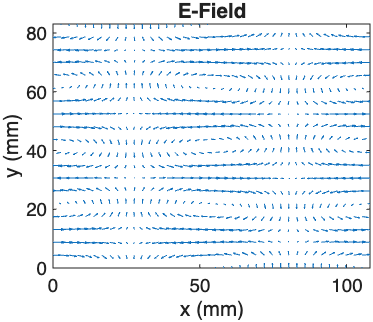
\includegraphics[width=\linewidth]{e.png}
        \caption{$E$ component }
    \end{subfigure}
    \hfill
    \begin{subfigure}[b]{0.35\linewidth}
        \centering
        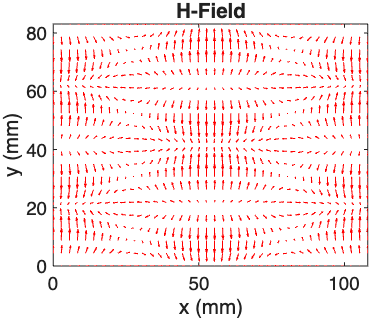
\includegraphics[width=\linewidth]{h.png}
        \caption{$H$ component}
    \end{subfigure}
    

         \centering
    \vspace{0.5cm}

    \begin{subfigure}[b]{0.35\linewidth}
        \centering
        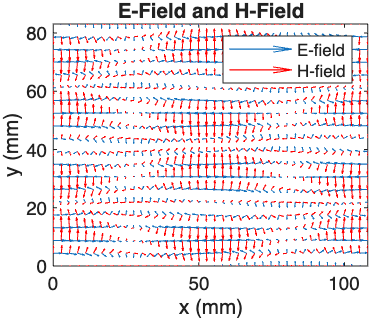
\includegraphics[width=\linewidth]{e and h.png}
        \caption{$E$ and $H$ components}
    \end{subfigure}
    \hfill
    \begin{subfigure}[b]{0.35\linewidth}
        \centering
        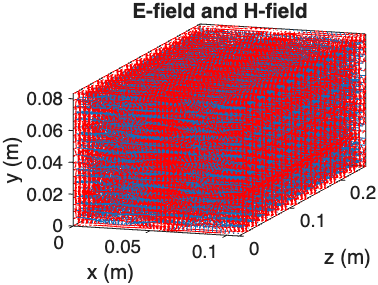
\includegraphics[width=\linewidth]{3d eand h.png}
        \caption{3D visualization of $E$ and $H$}
    \end{subfigure}
\end{figure}


  \begin{figure}[H]  
    \begin{subfigure}[b]{0.4\linewidth}
        \centering
        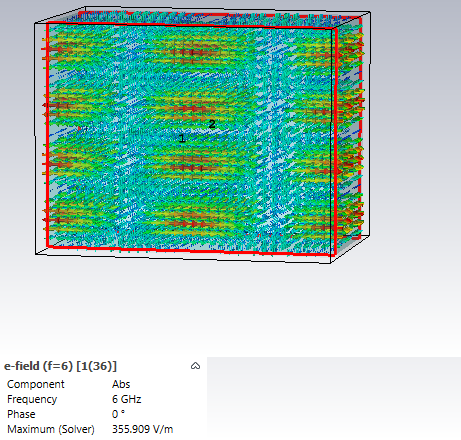
\includegraphics[width=\linewidth]{e-field (f=6) [1(36)].png}
        \caption{visualization of $E$ for TE$_{2,4}$}
    \end{subfigure}
    \hfill
    \begin{subfigure}[b]{0.4\linewidth}
        \centering
        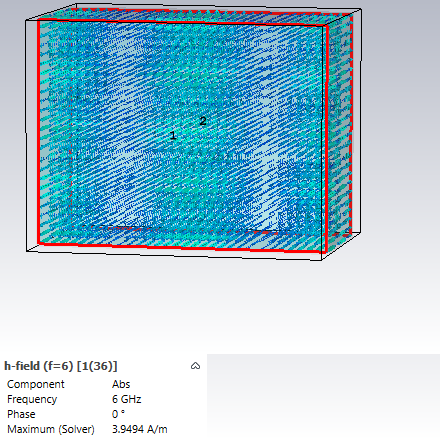
\includegraphics[width=\linewidth]{h-field (f=6) [1(36)].png}
        \caption{ visualization of $H$ for TE$_{2,4}$}
    \end{subfigure}

    \caption{Electric and magnetic field distributions of the TE$_{2,4}$ mode from MATLAB and CST.}
    \label{fig:fields}
\end{figure}

\subsection{Surface Current Density and Power Flow}
\begin{figure}[H]
    \centering
    \begin{subfigure}[b]{0.45\linewidth}
        \centering
        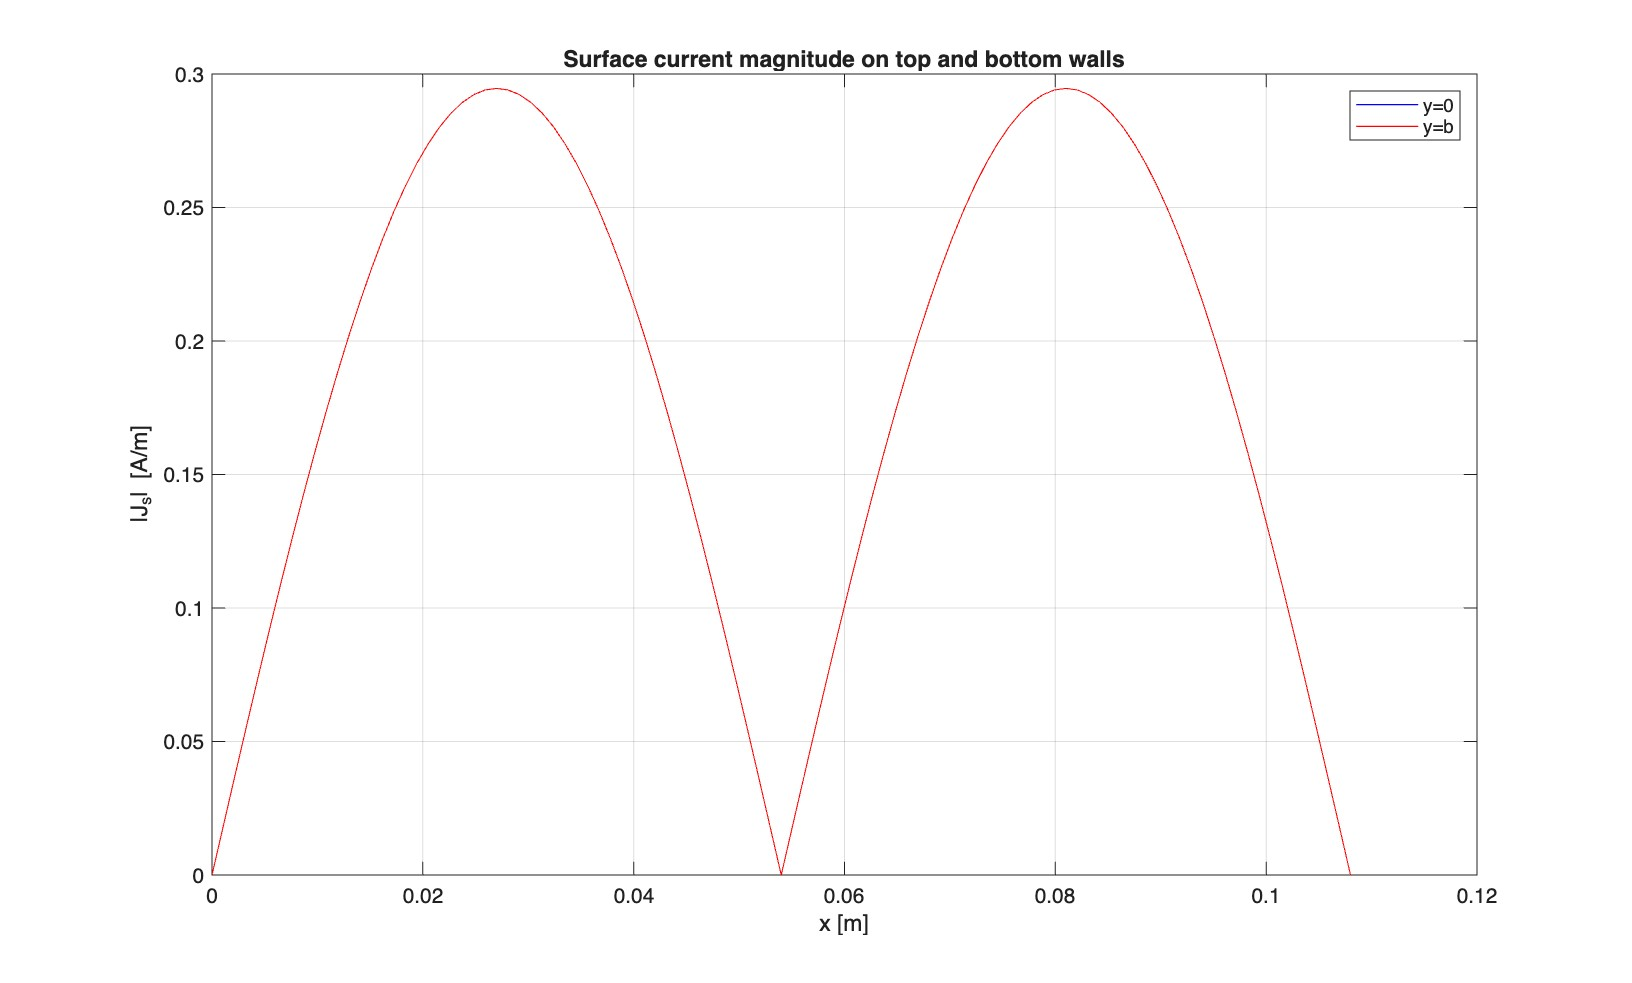
\includegraphics[width=\linewidth]{j top.jpg}
        \caption{Current density on the top and bottom surfaces}
    \end{subfigure}
    \hfill
    \begin{subfigure}[b]{0.45\linewidth}
        \centering
        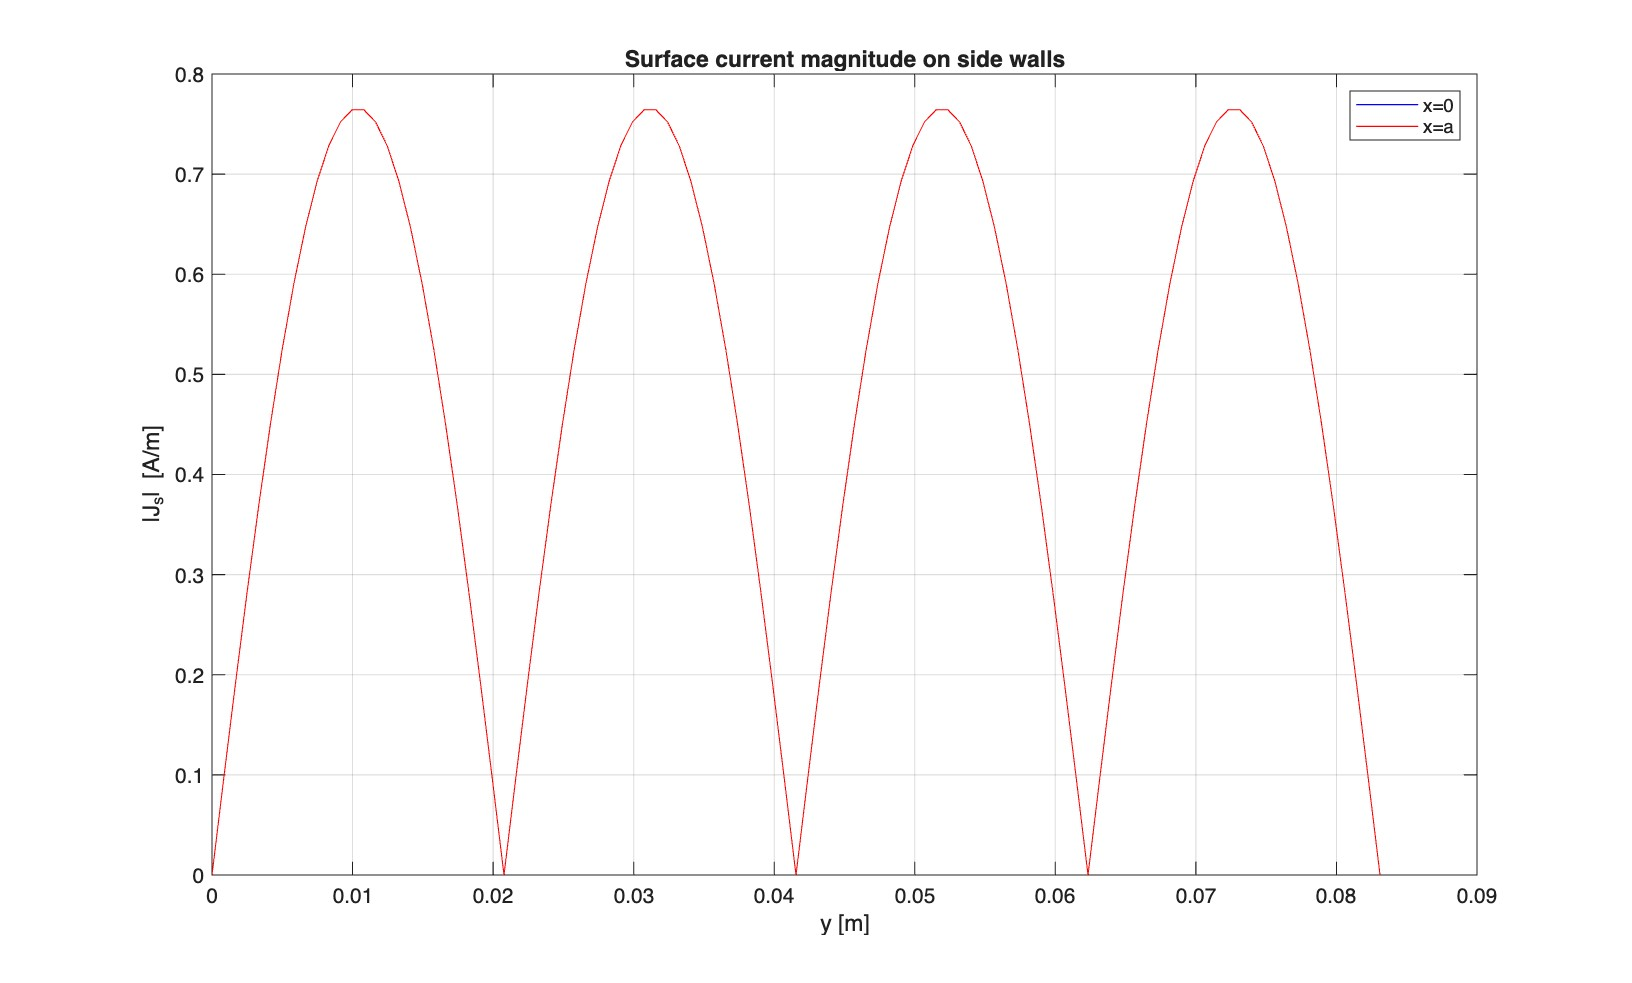
\includegraphics[width=\linewidth]{j left .jpg}
        \caption{Current density on the left and right surfaces}
    \end{subfigure}
    
    \vspace{0.5cm}

    \begin{subfigure}[b]{0.45\linewidth}
        \centering
        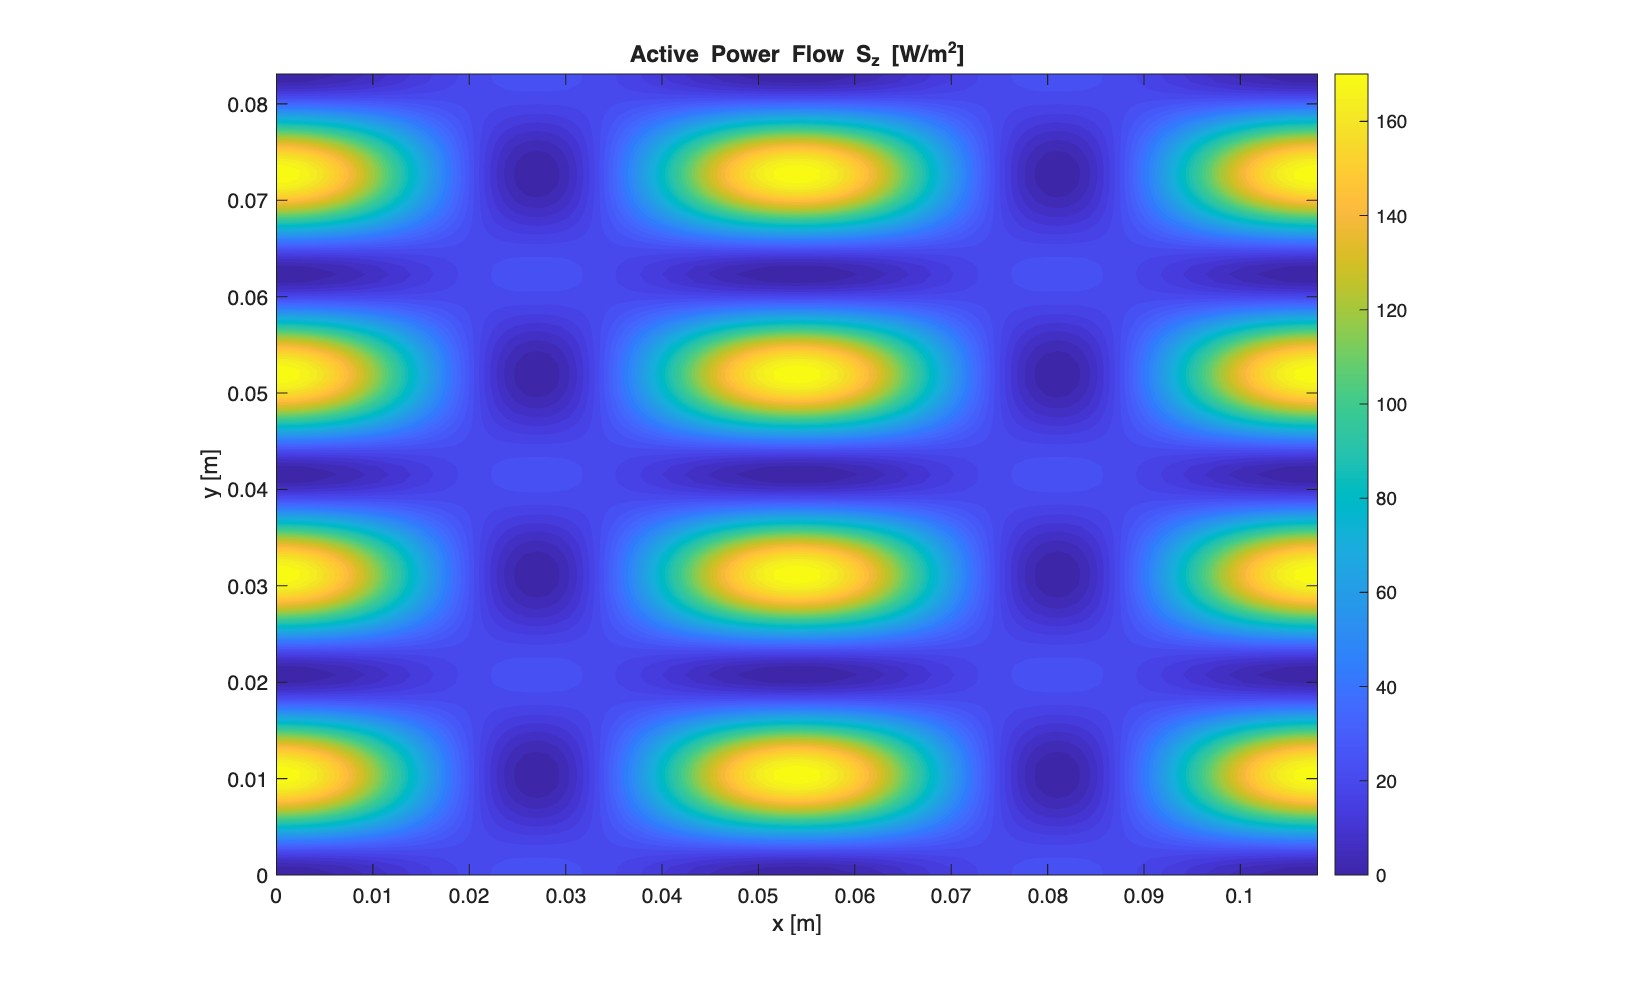
\includegraphics[width=\linewidth]{s.jpg}
        \caption{Power flow distribution}
    \end{subfigure}
\end{figure}

\begin{figure}[H]
    \centering
    \begin{subfigure}[b]{0.4\linewidth}
        \centering
        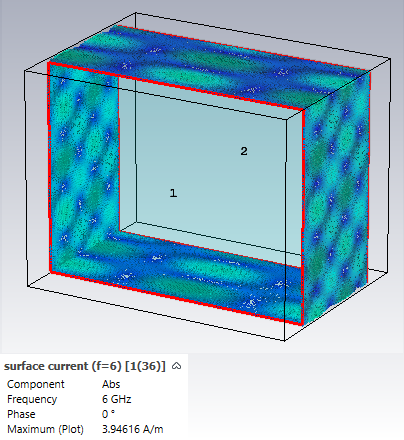
\includegraphics[width=\linewidth]{surface current (f=6) [1(36)]_1.png}
        \caption{surface current density(CST)}
    \end{subfigure}
    \hfill
    \begin{subfigure}[b]{0.45\linewidth}
        \centering
        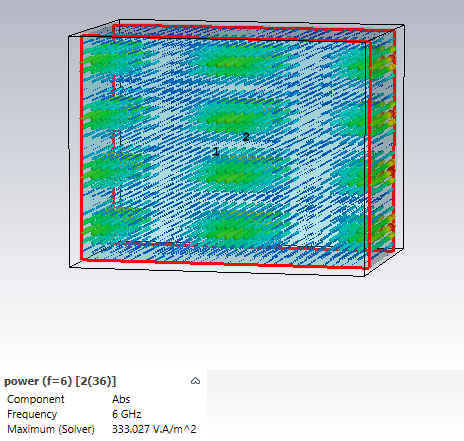
\includegraphics[width=\linewidth]{power_f.png}
        \caption{Power Visualization(CST)}
    \end{subfigure}
    
    
\end{figure}

From the simulations performed using \textsc{Matlab} and \textsc{CST}, it can be observed that the results visually agree well. The cutoff frequency $f_c$ for the $\text{TE}_{2,4}$ mode is $4.463~\text{GHz}$ in \textsc{Matlab} and $4.459~\text{GHz}$ in \textsc{CST}$,$ showing a difference of less than $0.1\%,$ which indicates accuracy and consistency between the analytical and simulated results.

\section{ Frequency-Dependent Parameters}
For $1.2 f_c < f < 1.8 f_c$:
\begin{align*}
\beta &= k_0 \sqrt{1 - \left(\frac{f_c}{f}\right)^2}, \quad
v_p = \frac{c}{\sqrt{1 - \left(\frac{f_c}{f}\right)^2}}, \quad
v_g = c \sqrt{1 - \left(\frac{f_c}{f}\right)^2}, \\
Z_{TE} &= \frac{\eta_0}{\sqrt{1 - \left(\frac{f_c}{f}\right)^2}}, \quad
\lambda_g = \frac{\lambda_0}{\sqrt{1 - \left(\frac{f_c}{f}\right)^2}}
\end{align*}

\begin{figure}[H]
    \centering
    \begin{subfigure}[b]{0.45\linewidth}
        \centering
        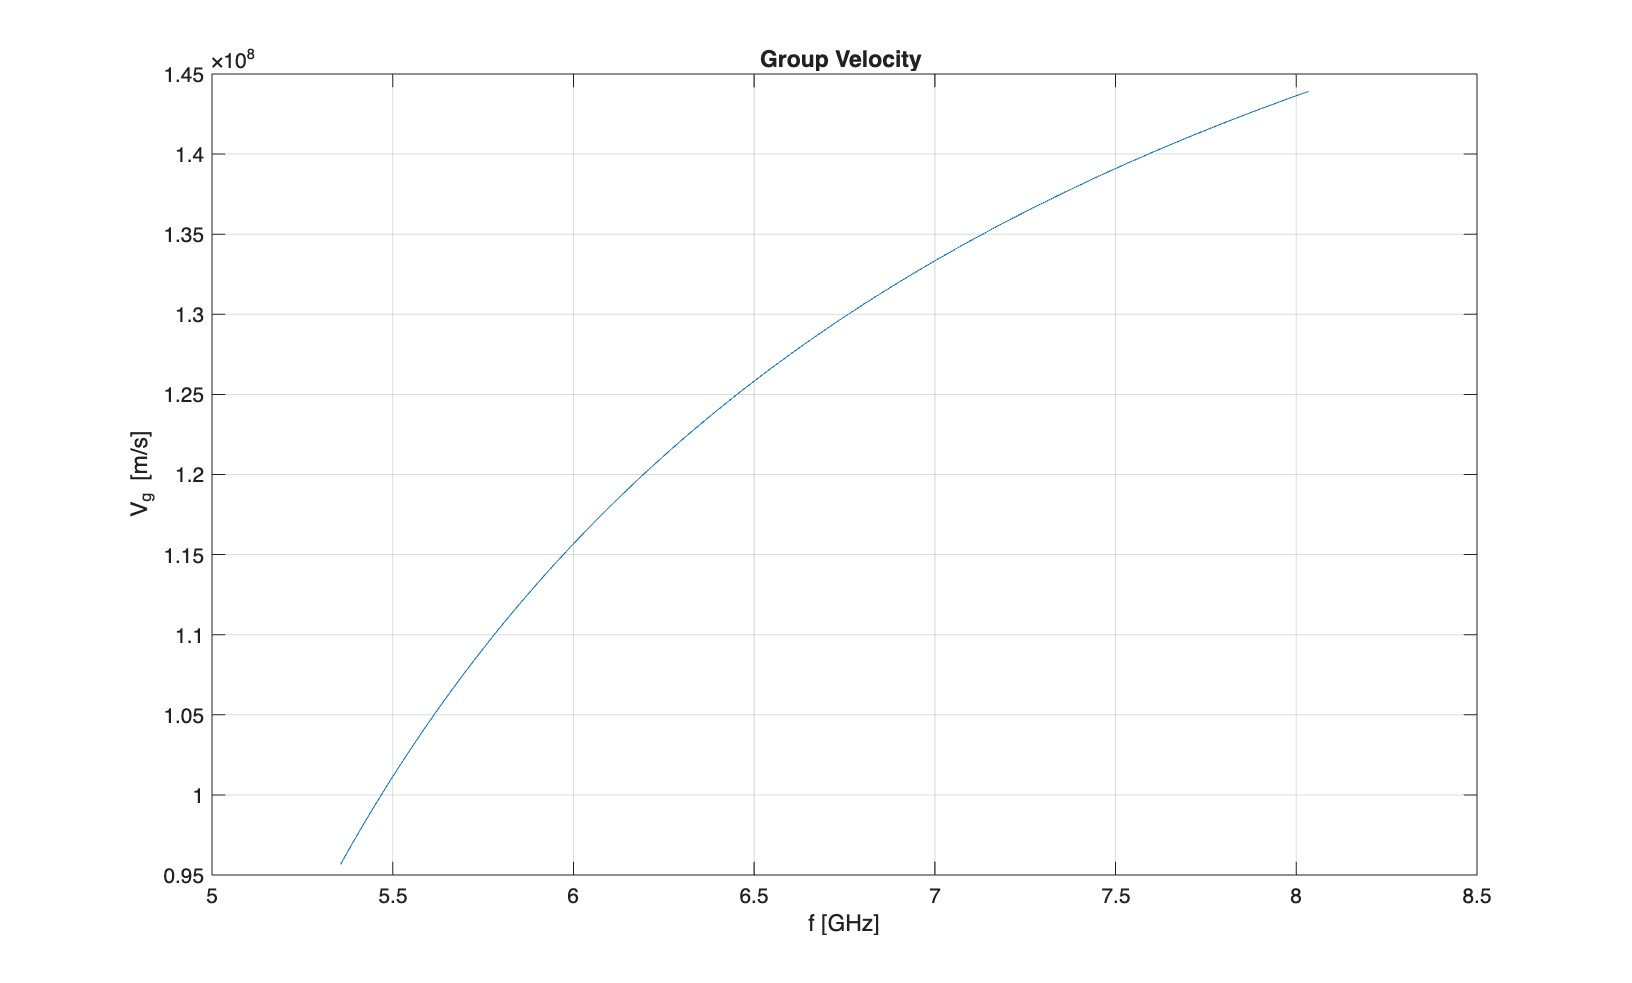
\includegraphics[width=\linewidth]{vg.jpg}
        \caption{Group Velocity}
    \end{subfigure}
    \hfill
    \begin{subfigure}[b]{0.45\linewidth}
        \centering
        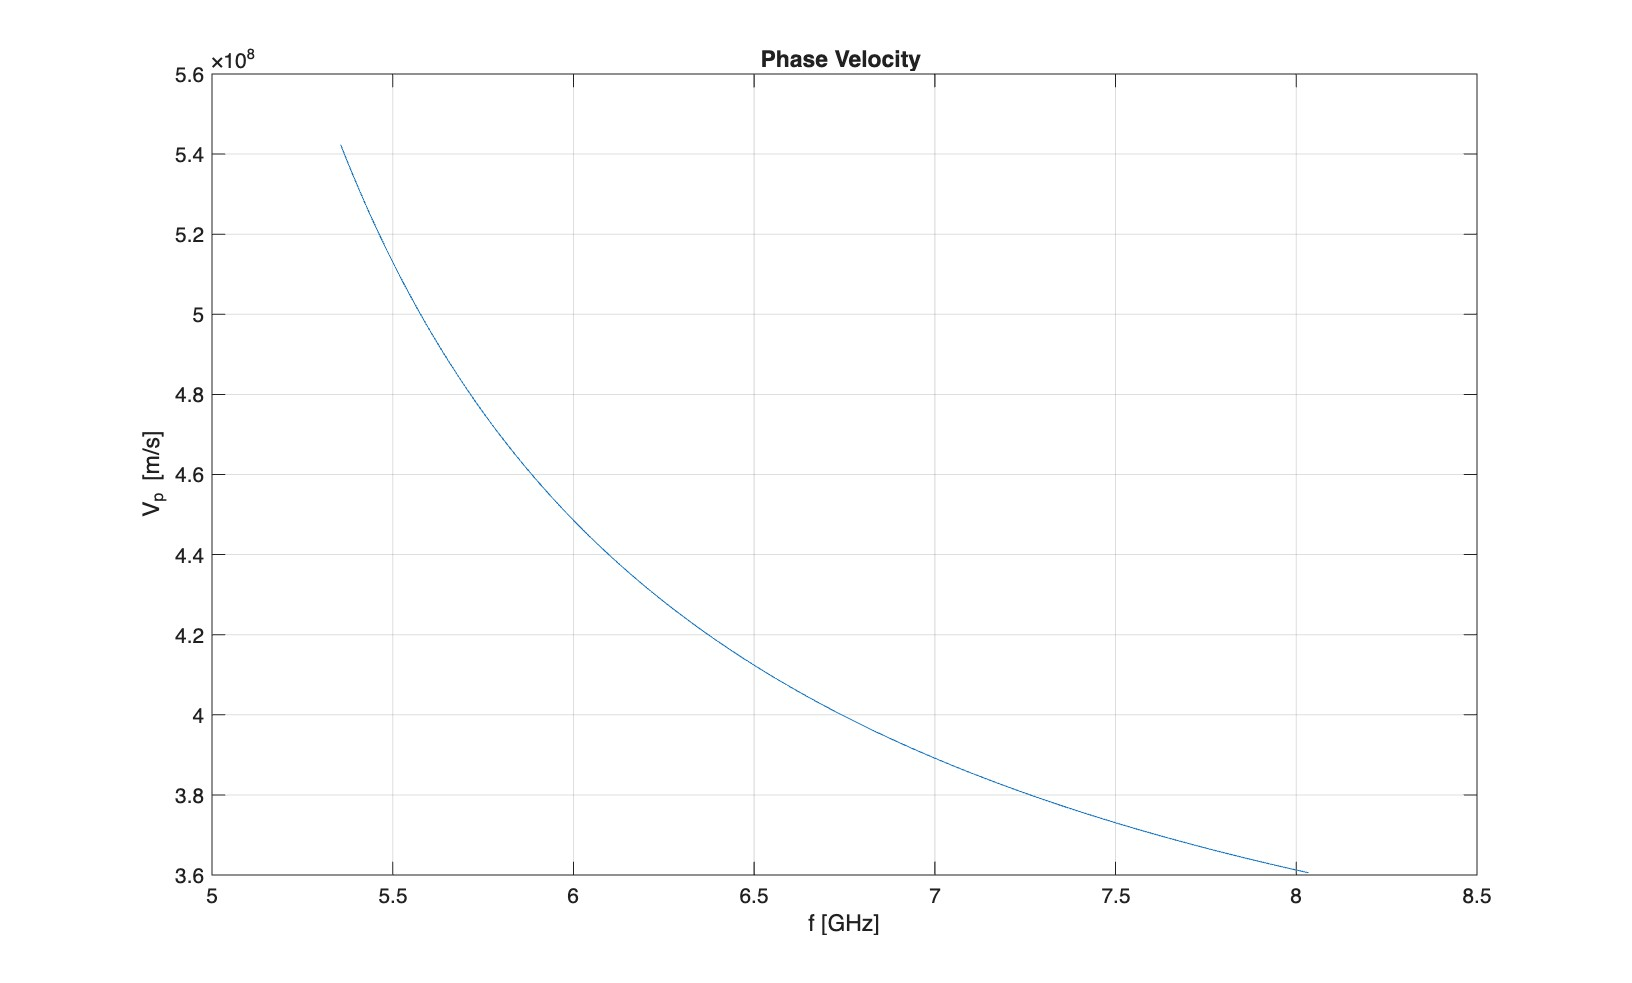
\includegraphics[width=\linewidth]{vp.jpg}
        \caption{Phase Velocity}
    \end{subfigure}
    \end{figure}
    \hfill
    \begin{figure}[H]
    \begin{subfigure}[b]{0.45\linewidth}
        \centering
        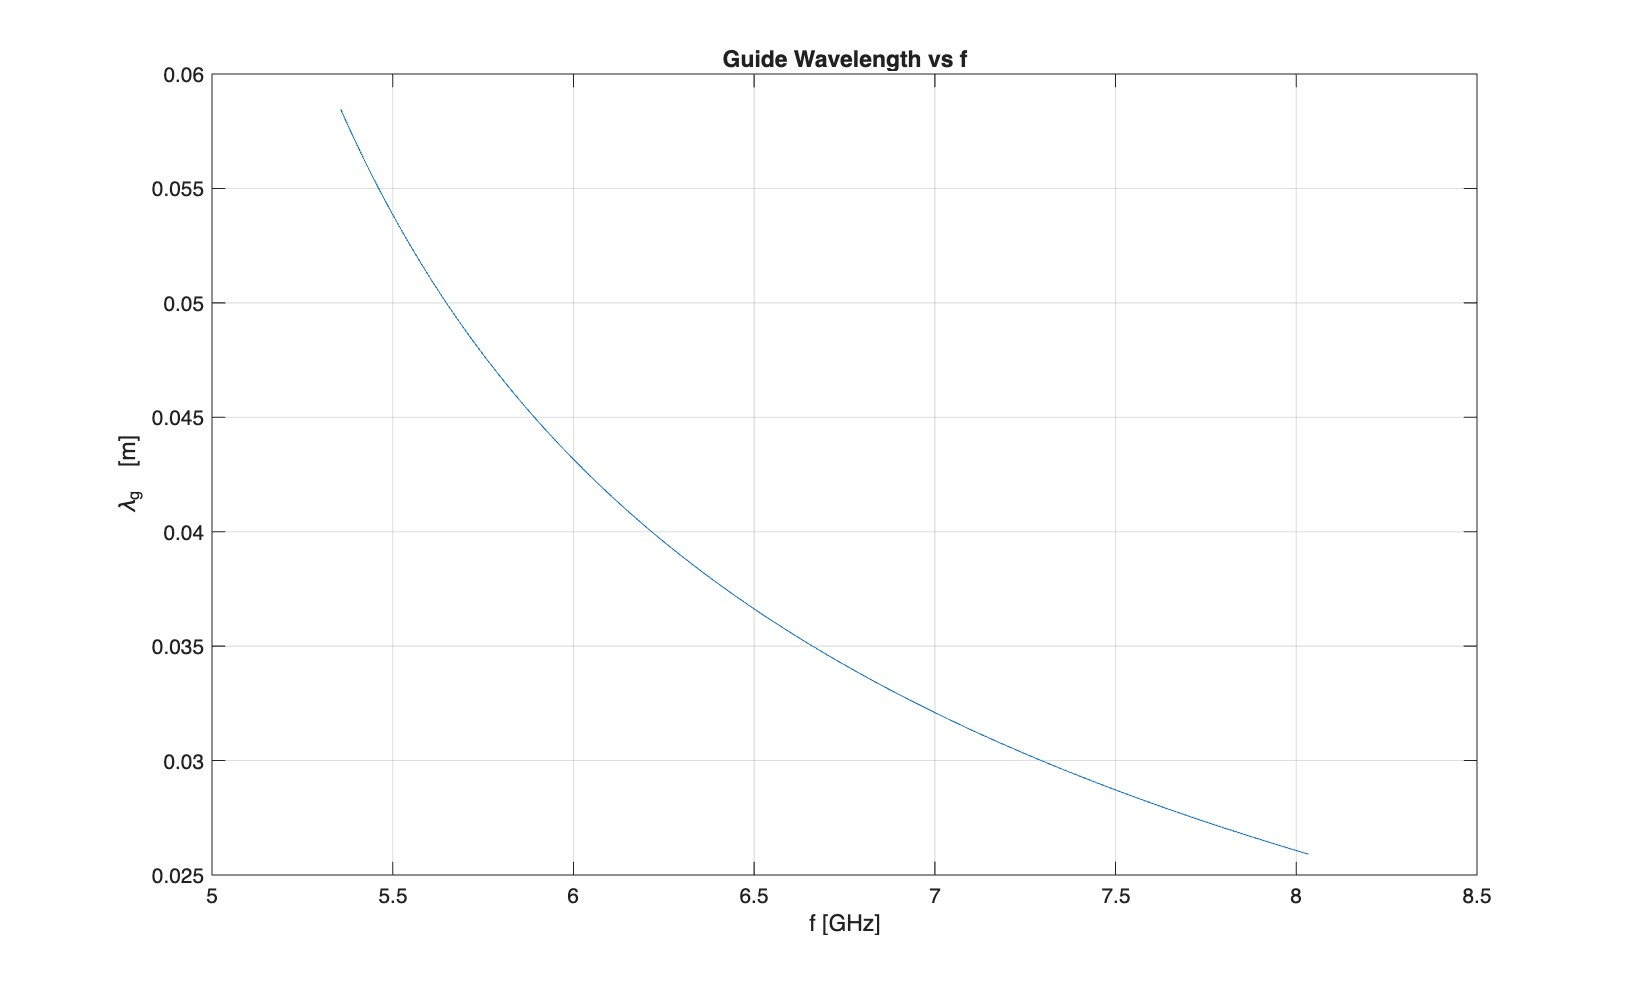
\includegraphics[width=\linewidth]{lambda.jpg}
        \caption{Waveguide Wavelength}
    \end{subfigure}
    \hfill
    \begin{subfigure}[b]{0.45\linewidth}
        \centering
        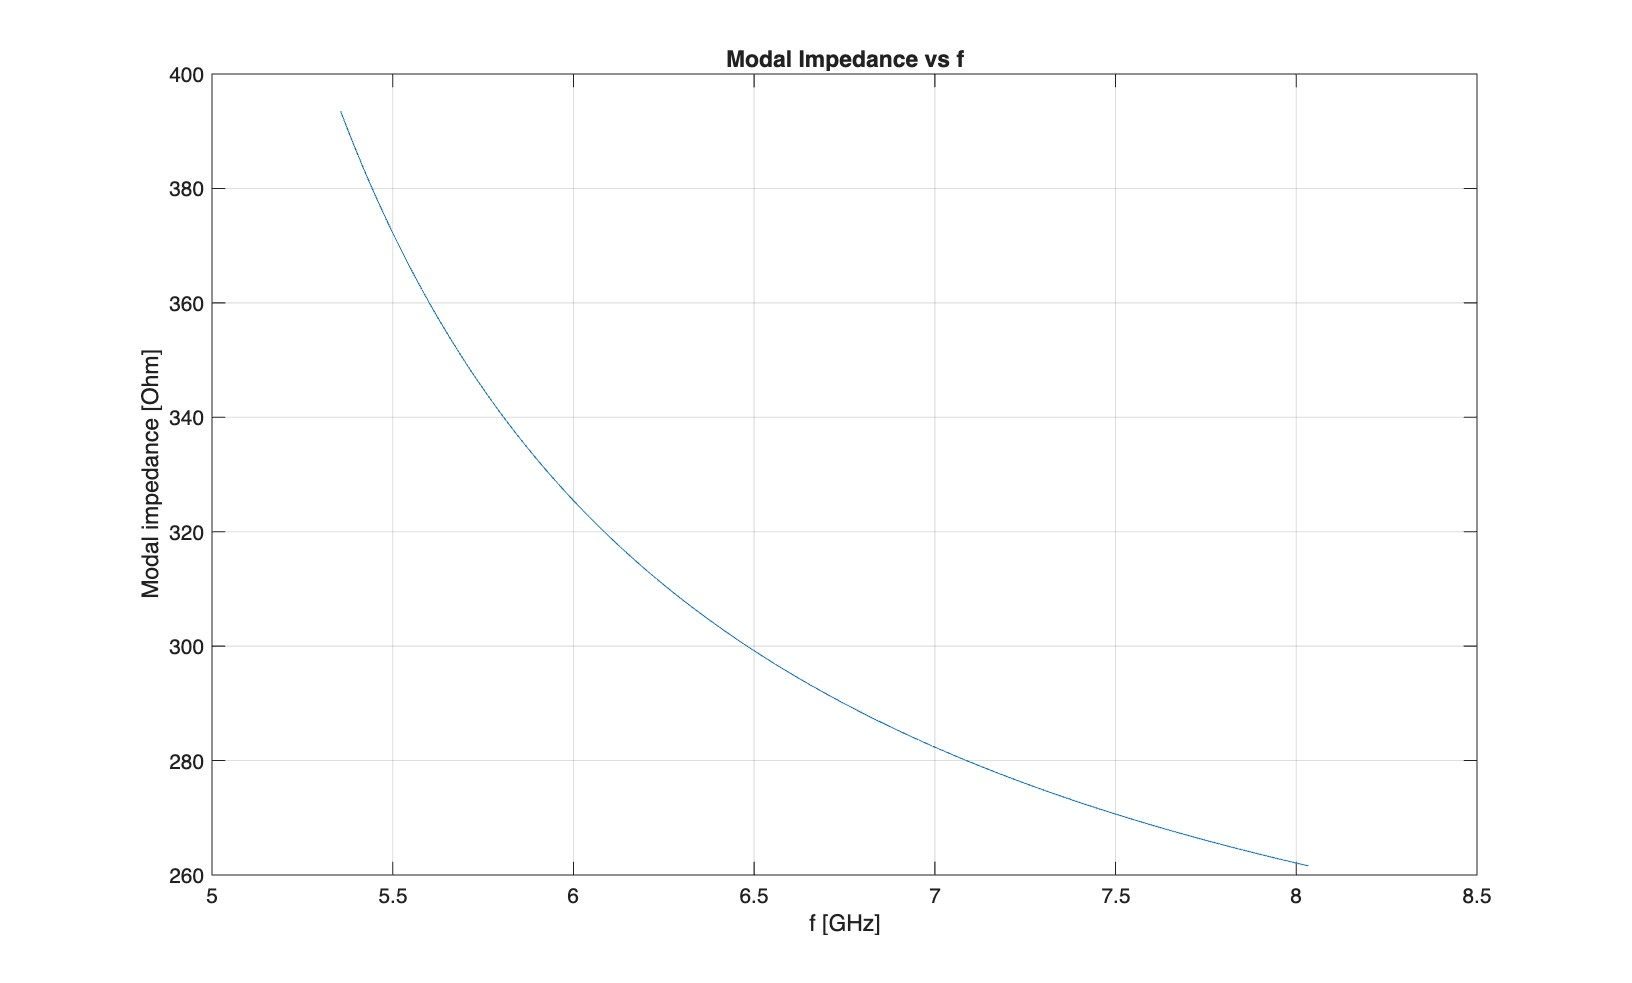
\includegraphics[width=\linewidth]{imoedance.jpg}
        \caption{Modal Impedance}
    \end{subfigure}
    \caption{Frequency-dependent parameters of the rectangular waveguide.}
\end{figure}


\section{Differential Delay TE$_{1,0}$ (Fastest) vs TE$_{2,4}$}

The differential delay over $L = 90$ m is the reason for using $v_g$ rather than $v_p$. Since we are dealing with signals that are propagating in the waveguide, $v_g$ has been chosen because it shows how fast the energy or information is traveling, rather than the phase of one frequency component.



\[
\Delta \tau = L \left( \frac{1}{v_{g,\text{TE}_{2,4}}} - \frac{1}{v_{g,\text{TE}_{1,0}}} \right)
\]


\begin{figure}[H]
    \centering
    \begin{subfigure}[b]{0.35\linewidth}
        \centering
        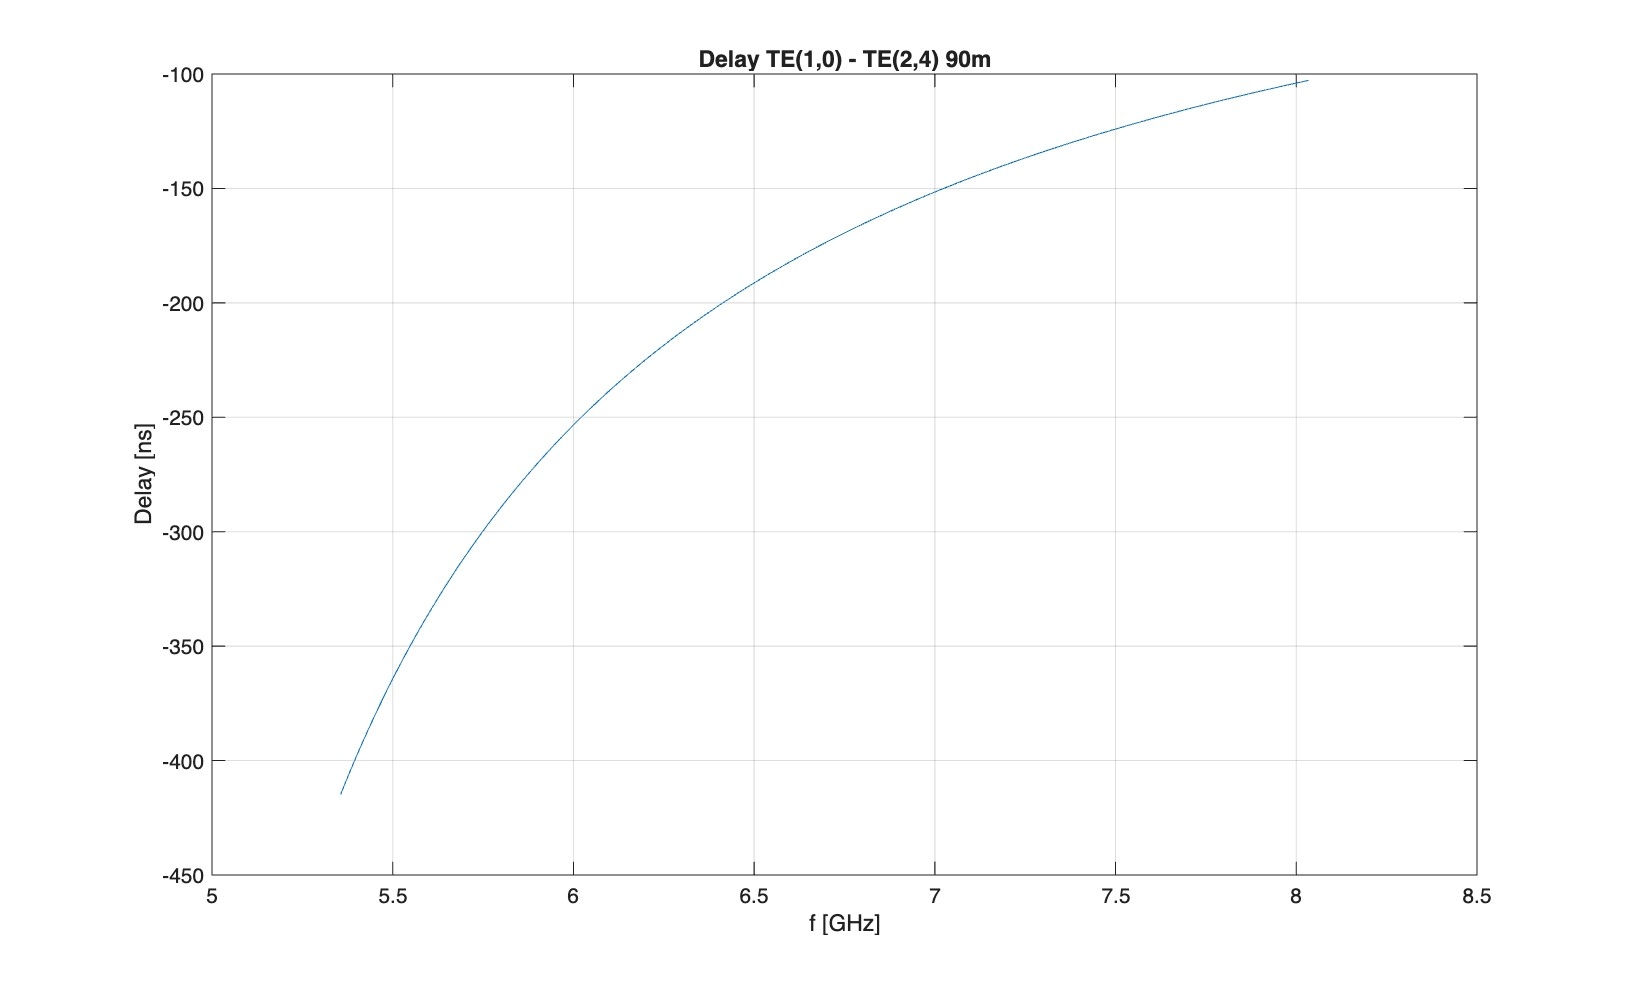
\includegraphics[width=\linewidth]{delay1.jpg}
        \caption{$E$ component}
    \end{subfigure}
\end{figure}

\section{ Differential Delay TE$_{2,4}$ vs TE$_{1,4}$}
Similarly:
\[
\Delta \tau= L \left( \frac{1}{v_{g,\text{TE$_{1,4}$}}} - \frac{1}{v_{g,\text{TE$_{2,4}$ }}} \right)
\]

\begin{figure}[H]
    \centering
    \begin{subfigure}[b]{0.35\linewidth}
        \centering
        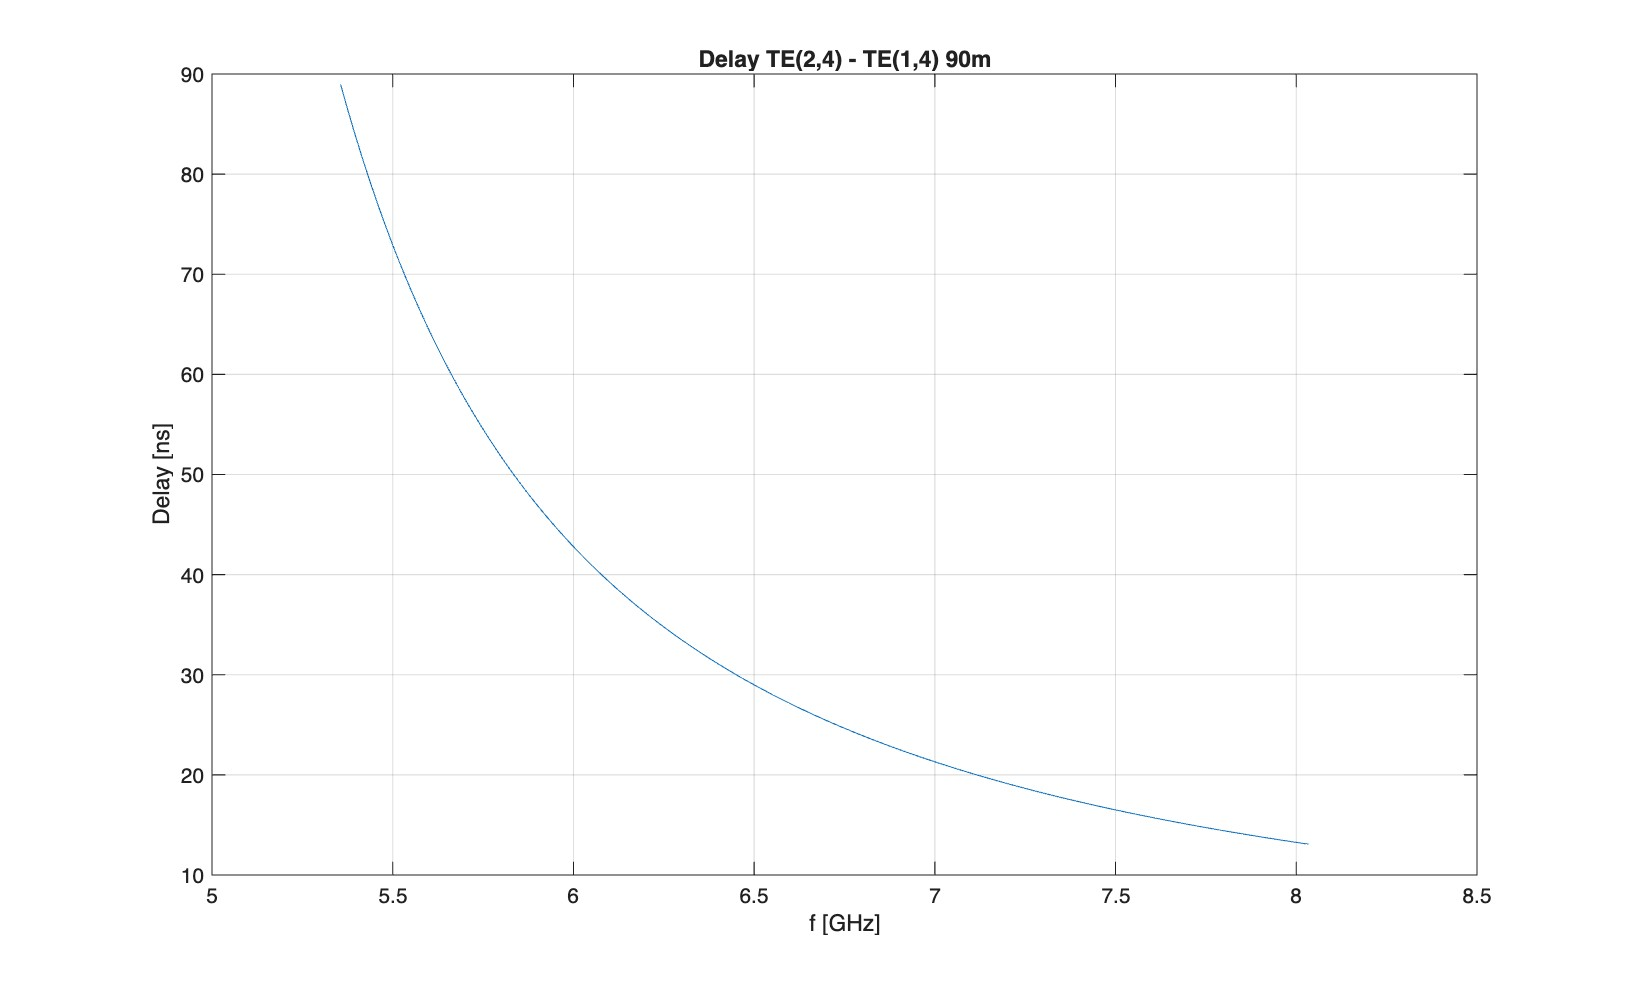
\includegraphics[width=\linewidth]{delay2.jpg}
        \caption{$E$ component}
    \end{subfigure}
\end{figure}


\section{Modal Filter Design}
The design of the modal filter is based on numerical calculations of the electric field for the TE$_{2,4}$ mode. By introducing an electric wall, the $E_x$ component of the electric field is canceled along the $x$ direction, while $E_y$ remains non-zero, allowing propagation at $x = a/2$. From this condition, one constraint on $m$ can be determined by solving the field equations in reverse for $x = a/2$, yielding $m = 2, 4, 6, 8$. 

Furthermore, by considering the surface current density from the magnetic field equations, it can be deduced that a cut along the $z$-axis at $x = a/4$ will preserve the mode while canceling the components of the current along the direction orthogonal to the cut, which is $x$, corresponding to $m = 2, 6, 10$.


Consequently, the modes that continue to propagate through the structure are 
TE$_{2,0}$, TE$_{2,1}$, TM$_{2,1}$, TE$_{2,2}$, TM$_{2,2}$, TE$_{2,4}$, and TM$_{2,4}$. 
These modes satisfy the boundary conditions imposed by both the PEC wall and the slot, 
while other modes are effectively suppressed.

\begin{figure}[H]
    \centering
    \begin{subfigure}[b]{0.4\linewidth}
        \centering
        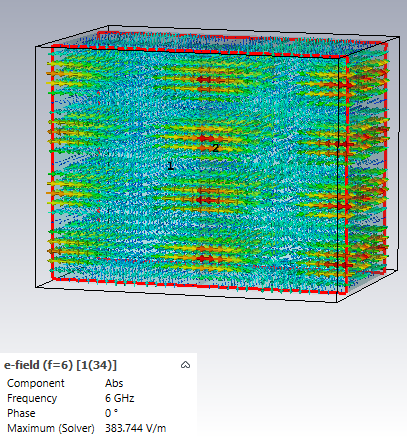
\includegraphics[width=\linewidth]{e-field (f=6) [1(34)].png}
        \caption{$E$ component after the inserting the PEC wall}
    \end{subfigure}
\end{figure}






\begin{figure}[H]
    \centering
    \begin{subfigure}[b]{0.45\linewidth}
        \centering
        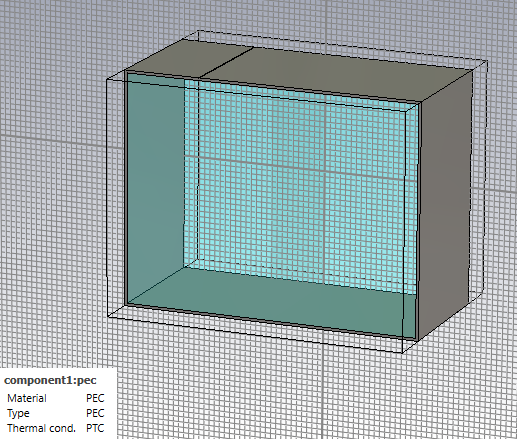
\includegraphics[width=\linewidth]{3D.png}
        \caption{Thin slot located at $x = a/4$}
    \end{subfigure}
    \hfill
    \begin{subfigure}[b]{0.45\linewidth}
        \centering
        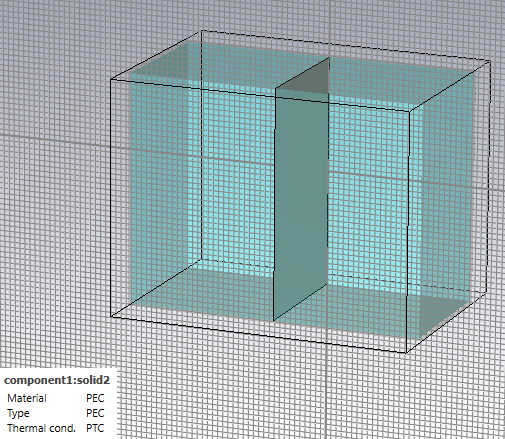
\includegraphics[width=\linewidth]{3D_1.png}
        \caption{PEC wall loacted at $x = a/2$ }
    \end{subfigure}
    \end{figure}
   



















\end{document}


